\appendix
\section{Dynamic Calculations}
\label{appendix}

To estimate a response time we pose the differential equation:

\begin{equation}
    m^* \ddot{x}(t) = -kx(t) + F_{ES}(x(t))
    \label{eq:diff_equation}
\end{equation}

The equation (\ref{eq:effective_mass}) describes the effective mass $m^*$.
The electro static force $F_{ES}$ depends on the square of the distance as seen in equation (\ref{eq:electrostatic_force}), which makes (\ref{eq:diff_equation}) a \emph{non-linear} ordinary differential equation.
We aren't going to solve a non-linear differential equation.
If we use the \emph{first order Taylor approximation} of $F_{ES}$ instead, we get an equation of the form $m^* \ddot{x}(t) = (\dot{F}_{ES}(0) - k) x(t) + F_{ES}(0)$ and the term $\dot{F}_{ES}(0)$ is negligible in comparison to $k$ when the actuator pad doesn't get too close to the ground pad when the switch is in the \emph{on} position.
So we solve equation (\ref{eq:diff_equation_lin}) to finally get a conservative estimate of the response time.

\begin{equation}
    m^* \ddot{x}(t) = -kx(t) + F_{ES}(0)
    \label{eq:diff_equation_lin}
\end{equation}

Using the \emph{Laplace method} we get the solution $x(t) = \frac{F}{k}\left[1-\cos{\left(\sqrt{\frac{k}{m}}t\right)}\right]$, which we can solve for $t$ to get (\ref{eq:switching_time}), which yields an estimation of the time it takes for the beam to go from its resting position to the \emph{on} position.

\begin{equation}
    t_{on} = \sqrt{\frac{m*}{k}} \cos^{-1}{\left( 1 - \frac{k x_{gap}}{F_{ES}} \right)} 
    \label{eq:switching_time}
\end{equation}

The equation (\ref{eq:switching_time}) is only defined for $k x_{gap} < F_{ES}$, because otherwise the applied force wouldn't be strong enough for the beam to reach the contact pad.
In the valid range of $0 < k < F_{ES}/x_{gap}$, the minimal switching time lies at $k = 0$.

So, a minimal spring constant $k$ would be favorable for a fast response time.
However, we can't apply a force that pushes the cantilever back to its initial position, thus we'd like a high \emph{resonance frequency} to get a fast response time when switching \emph{off}.
The resonance frequency requires a high spring constant for it to be high (equation~\ref{eq:resonance_frequency}).
There's a trade-off between the switching times in either directions for an optimal over-all switching frequency, which we can pose as an optimization problem (\ref{eq:switching_time_optimization}).

\begin{equation}
    k_{optimal} = \arg\min_k \left[ t_{on}(k) + t_{off}(k) \right] = \arg\min_k \sqrt{\frac{m^*}{k}} \left[ \frac{1}{2\pi} + \cos^{-1}{\left( 1 - \frac{k x_{gap}}{F_{ES}} \right)} \right]
    \label{eq:switching_time_optimization}
\end{equation}

Unfortunately, (\ref{eq:switching_time_optimization}) is non-trivial to solve.
Also, the effective mass $m^*$ depends on the same parameters as $k$, which makes (\ref{eq:switching_time_optimization}) technically incorrect and problem even harder to solve.
But we know that the optimum isn't at $k=0$ nor $k=F_{ES}/x_{gap}$ (either end of the valid range).

\newpage
\section{ANSYS}
\lstset{basicstyle=\footnotesize\ttfamily,breaklines=true}
\lstinputlisting{../src/beam_air.txt}

\begin{figure}[h]
	\centering
	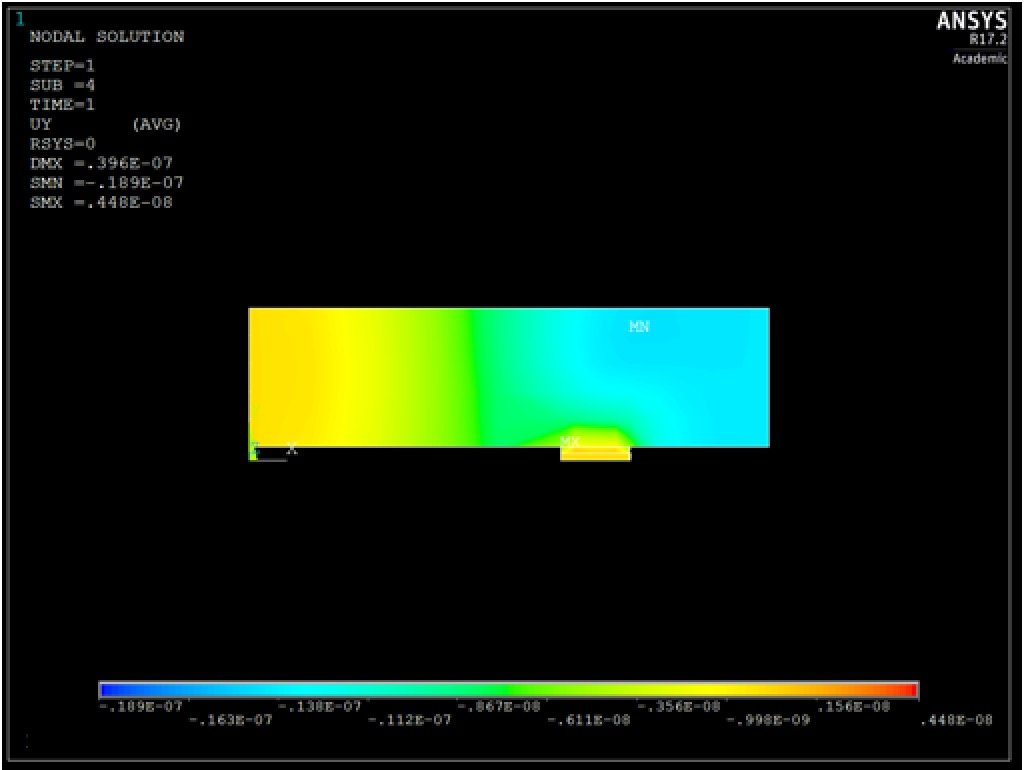
\includegraphics[width=\linewidth]{fig/ansys_beam.jpg}
	\label{fig:cantilever_beam}
\end{figure}
